\renewcommand{\theequation}{\theenumi}
\begin{enumerate}[label=\arabic*.,ref=\thesubsection.\theenumi]
\numberwithin{equation}{enumi}
%\chapter{The Optimum Receiver}
%\item Angles opposite to equal sides of a triangle are equal. 
%\label{prob:tri_ang_side_eq}
%\\
%\solution Using the sine formula in \eqref{eq:tri_sin_form},%
%\begin{align}
%\frac{\sin A}{a} = \frac{\sin B}{b}
%\end{align}
%%
%Thus, if $A=B$, $\sin A = \sin B \implies a =b$.
%\\
%\solution Use \eqref{eq:tri_sin_form} and the argument in Problem \ref{prob:tri_ang_side_eq}
%
\item  Each angle of an equilateral triangle is of 60$\degree$. 
	\iffalse
\\
\solution 
\begin{enumerate}
\begin{figure}[!ht]
\centering
\resizebox{\columnwidth}{!}{\begin{tikzpicture}
[scale=2,>=stealth,point/.style={draw,circle,fill = black,inner sep=0.5pt},]

%Triangle sides
\def\a{4}
\def\b{4}
\def\c{4}
 
%Coordinates of A
\def\p{2}
\def\q{{sqrt(\c^2-\p^2)}}

%Labeling points
\node (A) at (\p,\q)[point,label=above right:$A$] {};
\node (B) at (0, 0)[point,label=below left:$B$] {};
\node (C) at (\a, 0)[point,label=below right:$C$] {};

%Drawing triangle ABC
\draw (A) -- node[left, xshift=-5mm,yshift=5mm] {$\textrm{a}$} (B) -- node[below, yshift=-5mm] {$\textrm{a}$} (C) -- node[above right,xshift=2mm,yshift=5mm] {$\textrm{a}$} (A);


%Angles
\tkzFillAngle[fill=green!60,size=.5](C,B,A)

%
\tkzFillAngle[fill=red!60,size=.5](A,C,B)

%%
\tkzFillAngle[fill=orange!60,size=.5](B,A,C)
%
%\tkzFillAngle[fill=blue!60,size=.3](E,A,F)
\end{tikzpicture}

}
\caption{}
\label{fig:8.1.1_similar}	
\end{figure}


\item {\em Construction: } See Fig. \ref{fig:8.1.1_similar}.
The input parameters are
\begin{multline}
 \vec{B}= \myvec{0\\0},
\vec{C}=\myvec{a\\0},
\vec{A}=a\myvec{\cos 60\degree\\ \sin 60\degree}
\end{multline}

\item {\em Proof: } Using the cosine formula,
%
\begin{align}
\cos \phase{ABC} &= \frac{a^2 +a^2 - a^2}{2a^2}
\\
&= \frac{1}{2}
\\
\implies  \phase{ABC} &= 60 \degree
\end{align}
%


\end{enumerate}
\fi
%%
%\begin{align}
%A=B=C.&
%\\
%\because A+B+C = 180\degree, 3A = 180\degree&
%\\
%\implies A = 60\degree&
%\end{align}
%


%\subsection{Problem}
\item Triangles on the same base (or equal bases) and between the same parallels are equal in area.
	\iffalse
\begin{enumerate}
\begin{figure}[!ht]
\centering
\resizebox{\columnwidth}{!}{\begin{tikzpicture}[scale = 1.5,>=stealth,point/.style={draw,circle,fill=black, inner sep=0.5pt},]

\node (A) at (2,0)[point,label=below:$A$] {};
\node (B) at (5,0)[point,label=below:$B$] {};
\node (C) at (3,2)[point,label=above:$C$] {};
\node (D) at (4,2)[point,label=above:$D$] {};
\node (E) at (0,0)[] {};
\node (F) at (7,0)[] {};
\node (G) at (0,2)[] {};
\node (H) at (7,2)[] {};
\node (M) at (3,0)[point,label=below:$M$] {};
\node (N) at (4,0)[point,label=below:$N$] {};

\draw (A) -- node[below=5pt]{}(B) -- (C) -- (A);
\draw (A) -- node[below=5pt]{}(B) -- (D) -- (A);
\draw (E) -- node[below=5pt]{}(F);
\draw (G) -- node[below=5pt]{}(H);
\draw[dotted] (C) -- node[below=5pt]{}(M);
\draw[dotted] (D) -- node[below=5pt]{}(N);

\tkzMarkRightAngle[fill=blue!20, mark=|](C,M,A)
\tkzMarkRightAngle[fill=blue!20, mark=|](D,N,A)
\end{tikzpicture}}
\caption{}
\label{fig:8.1.2_triangle1}	
\end{figure}

\item {\em Construction: }See  Fig. \ref{fig:8.1.2_triangle1}.  The design parameters are
\begin{align}
\vec{A} &= \myvec{0\\0}, 
\vec{B} = \myvec{a\\0}, 
\\
\vec{C} &= \myvec{p\\q}, p < a,\quad
\vec{D} &= \myvec{d\\q}, p < d < a
\end{align}



\item {\em Proof: } In Fig. \ref{fig:8.1.2_triangle1}, 
\begin{align}
ar\brak{\triangle ABC} = \frac{1}{2}aq = ar\brak{\triangle ABD}
\end{align}

\end{enumerate}
\fi
\item Triangles on the same base (or equal bases) and having equal areas lie between the same parallels.
\item In $\triangle ABC, D, E$ and $F$ are respectively the mid-points of sides $AB, BC$ and $CA $. Show that $\triangle ABC$ is divided into four congruent triangles by joining $D, E$ and $F$.
\item  The line-segment joining the mid-points of any two sides of a triangle is parallel to the third side and is half of it.
\label{prob:tri_mid_similar}
%\label{prob:quad_similar}
%%
%\\
%\solution If $DE$ is the lie joining he mid points of $\triangle ABC$,  use cosine formula to find the lengths of $DE$ and $BC$. Then use cosine formula to show that all angles of $\triangle ADE$ are equal to the corresponding angles of $\triangle ABC$.
%
\item  A line through the mid-point of a side of a triangle parallel to another side 
bisects the third side.
%\\
%\solution Use cosine formula.

\item ABC is a triangle right angled at $C$. A line through the mid-point $M$ of hypotenuse $AB$ and parallel to $BC$ intersects $AC$ at $D$. Show that (i) $D$ is the mid-point of $AC$
(ii) $MD \perp AC$ (iii) $CM = MA = \frac{1}{2}AB$

\item  Sides opposite to equal angles of a triangle are equal. 
%\\
%\solution Use \eqref{eq:tri_sin_form} and the argument in Problem \ref{prob:tri_ang_side_eq}
%
\item  Each angle of an equilateral triangle is of 60$\degree$. 
%\\
%\solution In an equilateral $\triangle$, 
%%
%\begin{align}
%A=B=C.&
%\\
%\because A+B+C = 180\degree, 3A = 180\degree&
%\\
%\implies A = 60\degree&
%\end{align}
%
\item Using cosine formula in an equilateral $\triangle$, show that $\cos 60\degree = \frac{1}{2} $.  
\item Using \eqref{eq:tri_sin_cos_id}, show that $\sin 60\degree = \frac{\sqrt{3}}{2} $.
\item Find  $\sin 30\degree$ and  $\sin 30\degree$ using \eqref{eq:tri_90-ang}.
%\subsection{Problem}
\item Triangles on the same base (or equal bases) and between the same parallels are equal in area.
\item Triangles on the same base (or equal bases) and having equal areas lie between the same parallels.
\item In $\triangle ABC$, the bisector $AD$ of $\angle  A$ is perpendicular to side $BC$. Show that $AB = AC$ and $\triangle ABC$ is isosceles.
\item $E$ and $F$ are respectively the mid-points of equal sides $AB$ and AC of $\triangle ABC$. Show that $BF = CE$. 
\item In an isosceles $\triangle ABC$ with $AB$ = AC, D and E are points on $BC$ such that $BE = CD$. Show that $AD = AE$. 
%
\item $AB$ is a line-segment. $P$ and $Q$ are points on opposite sides of $AB$ such that each of them is equidistant from the points $A$ and $B$. Show that the line $PQ $ is the perpendicular bisector of $AB$.
%
\item $P$ is a point equidistant from two lines $l$ and $m$ intersecting at point $A$.  Show that the line  $AP$  bisects the angle between them.
%
\item $D$ is a point on side $BC$ of $\triangle  ABC$ such that $AD = AC$. Show that $AB > AD$

%
\item $AB$ is a line segment and line $l$ is its perpendicular bisector. If a point $P$ lies on $l$, show that $P$ is equidistant from $A$ and $B$.
\item Line-segment $AB$ is parallel to another line-segment $CD$. $O$ is the mid-point of $AD$. Show that 
\begin{enumerate}
\item  $\triangle AOB \cong \triangle DOC$ 
\item  $O$ is also the mid-point of $BC$.
\end{enumerate}
%
\item In quadrilateral $ACBD, AC = AD$ and $AB$ bisects $\angle  A$. Show that $\triangle  ABC \cong \triangle  ABD$. What can you say about $BC$ and $BD$?
\label{prob:8.1.23}
\iffalse
\begin{enumerate}

\begin{figure}[!ht]
\centering
\resizebox{\columnwidth}{!}{\begin{tikzpicture}[scale=1.5,>=stealth,point/.style={draw,circle,fill = black,inner sep=0.5pt},]
      
%Labeling points
\node (A) at (0, 0)[point,label=below left:$A$] {};
\node (C) at (5, 0)[point,label=below right:$C$] {};
\node (B) at (7, 5.9)[point,label=above right:$B$] {};
\node (D) at (0.86, 4.92)[point,label=above left:$D$] {};
\node (O) at (1.95, 1.64)[point,label=above left:$O$] {};
\node (P1) at (1.95, 0)[point,label=below left:$P_1$] {};
\node (P2) at (0.33, 1.92)[point,label=above left:$P_2$] {};

%Drawing quad ABCD
\draw (A) -- node[below=5pt]{$\textrm{a}$}(C) -- (B) -- (D) -- (A);
\draw[dotted] (A) -- (B)(O) -- (P1) -- (P2) -- (O);

%marking angles
\tkzMarkRightAngle[fill=blue!20, mark=|](C,P1,O)
\tkzMarkRightAngle[fill=blue!20, mark=|](O,P2,D)
\tkzMarkAngle[fill=green!20, mark=|](B,A,D)
\tkzMarkAngle[fill=green!20, mark=|](C,A,B)

%marking lines
\tkzMarkSegment[color=black,pos=0.5,mark=s||](A,D)
\tkzMarkSegment[color=black,pos=0.5,mark=s||](A,C)

\end{tikzpicture}}
\caption{}
\label{fig:8.1.23_quad}	
\end{figure}
 
\item {\em Construxtion: }See  Fig. \ref{fig:8.1.23_quad}.  The input parameters are
%
\begin{align}
\vec{A} &=\myvec{0\\0} \label{eq:8.1.23_constr_a}\\
\vec{C} &= \myvec{a\\0}, \label{eq:8.1.23_constr_c}\\ 
\vec{D} &= a\myvec{\cos{\theta}\\\sin{\theta}}\label{eq:8.1.23_constr_b}
\end{align}
\subitem Let 
%
\begin{align}
\begin{split}
\vec{P}_1 &= \frac{\vec{C}}{\norm{ \vec{C} }} \\
\vec{P}_2 &= \frac{\vec{D}}{\norm{ \vec{D}}} 
\end{split}
 \label{eq:8.1.23_p1p2} 
\end{align}
If $AB$ be the angle bisector, it is easy to show that 
\begin{align}
P_1P_2 \perp  AB \\
\implies \brak{\vec{P}_1 - \vec{P}_2}^T \brak{\vec{B}-\vec{A}}
 \label{eq:8.1.23_Proofeq1} 
\end{align}
However, from  \eqref{eq:8.1.23_p1p2} ,
\begin{align}
\norm{ \vec{P}_1} &= \norm{ \vec{P}_2}  = 1\\
\implies \norm{ \vec{P}_1}^2 &= \norm{ \vec{P}_2}^2 
\\
\text{or, }\brak{\vec{P}_1-\vec{P}_2}^T\brak{\vec{P}_1+\vec{P}_2} &= 0 \\
\implies \vec{P}_1 + \vec{P}_2 \perp  \vec{P}_1-\vec{P}_2 \label{eq:8.1.23_Proofeq2}
\end{align}
From \eqref{eq:8.1.23_Proofeq1} and \eqref{eq:8.1.23_Proofeq2}
\begin{align}
\vec{B} &= \lambda\brak{\vec{P}_1+\vec{P}_2} 
\\
\implies \vec{B} &=  \lambda\brak{\frac{\vec{C}}{\norm{ \vec{C}}}+\frac{\vec{D}}{\norm{ \vec{D}}}}
\end{align}
when $\vec{A}$ is at the origin.  In general, 
\begin{align}
\vec{B} =  \vec{A} + \lambda\brak{\frac{\vec{C}-\vec{A}}{\norm{ \vec{C}-\vec{A}}}+\frac{\vec{D}-\vec{A}}{\norm{ \vec{D}-\vec{A}}}}
\end{align}
\item Using SAS congruence, it is trivial to show that $BC = BD$

$\triangle ABC \cong \triangle ABD$ by SAS congruence:
\begin{align*}
AD &= AC \\
\angle{DAB} &= \angle{BAC} \\
DB\ &is\ common
\end{align*}
$\implies BC = BD$
\end{enumerate}
\fi

%
\item $ABCD$ is a quadrilateral in which $AD = BC$ and $\angle  DAB = \angle  CBA$ . Prove that
\begin{enumerate}
\item  $\triangle  ABD \cong  \triangle  BAC $
\item $ BD = AC $
\item  $\angle  ABD = \angle  BAC$.
\end{enumerate}
%
\item $l$ and $m$ are two parallel lines intersected by another pair of parallel lines p and q 
to form the quadrilateral $ABCD$. Show that $\triangle  ABC \cong  \triangle  CDA$.
%
\item Line $l$ is the bisector of $ \angle  A$ and $B$ is any point on $l$. $BP$ and $BQ$ are perpendiculars from $B$ to the arms of $\angle  A$. Show that: 
\begin{enumerate}
\item  $\triangle  APB \cong  \triangle  AQB$ 
\item  $BP = BQ$ or $B$ is equidistant from the arms of $\angle  A$.
\end{enumerate}
%
\iffalse
\begin{enumerate}
\begin{figure}[!ht]
\centering
\resizebox{\columnwidth}{!}{

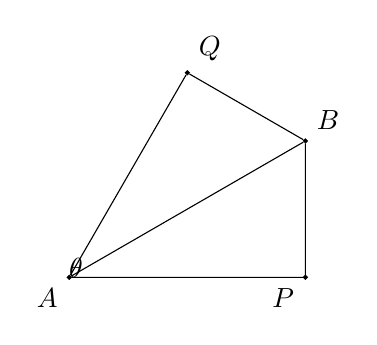
\begin{tikzpicture}
[scale=1,>=stealth,point/.style={draw,circle,fill = black,inner sep=0.5pt},]

\node (A) at (0,0)[point,label=below left:$A$] {};
\node (P) at (3, 0)[point,label=below left:$P$] {};
%\node (Q) at ($({3*\cos{60}}, {3*\sin{60}})$)[point,label=below right:$Q$] {};
%\node (B) at ($({3.4641*\cos{30}}, {3.4641*\sin{30}})$)[point,label=above right:$B$] {};
\node (Q) at (1.5, 2.598)[point,label=above right:$Q$] {};
\node (B) at (3, 1.732)[point,label=above right:$B$] {};




\draw (A) -- node[left] {$\textrm{}$} (P) -- node[below] {$\textrm{}$} (B) -- node[above,xshift=2mm] {$\textrm{}$} (Q);
\draw (A)--(Q);
\draw (A)--(B);


\tkzFillAngle[fill=green!40,size=0.4cm,mark=](P,A,B)
\tkzFillAngle[fill=orange!40,size=0.5cm,mark=](B,A,Q)
\tkzMarkRightAngle[fill=blue,size=.3](A,Q,B);
\tkzMarkRightAngle[fill=purple,size=.3](A,P,B);

%\tkzMarkRightAngle[fill=orange!40,size=0.4cm,mark=](A,Q,B)
%\tkzMarkRightAngle[fill=green!40,size=0.5cm,mark=](A,P,B)

\tkzLabelAngle[pos=0.7](P,A,Q){$\theta$}
%\tkzLabelAngle[pos=0.7](P,A,B){$\gamma$}


\end{tikzpicture}
}
\caption{ }
\label{fig:8.1.26_angle}	
\end{figure}

%\renewcommand{\thefigure}{\theenumi.\arabic{figure}}

\item {Construction: } See Fig. \ref{fig:8.1.26_angle}
The input parameters are
% 
\begin{align}
\vec{A} &= \myvec{0\\0},
\vec{P} &= \myvec{1\\0}
\vec{Q} &= \myvec{\cos \theta \\ \sin \theta}
\end{align}
resulting in 
% 
%
\begin{align}
\vec{B} &= \lambda{\vec{P}+\vec{Q}}
\\
\because \brak{\vec{B} - \vec{P}}^T \vec{P} &= 0,
\\
\brak{\lambda -1}+ \lambda \vec{Q}^T \vec{P} &=0
\end{align}
resulting in 
\begin{align}
\lambda = \frac{1}{1+\vec{P}^T \vec{Q} }
\end{align}



\item 	In Fig. \ref{fig:8.1.26_angle} using ASA congruence,
\begin{align}
\triangle APB &\cong \triangle AQB
\\
\implies BP = BQ
\end{align}

\end{enumerate}
\fi

\item $ABCE$ is a quadrilateral and $D$ is a point on $BC$ such that, $AC = AE, AB = AD$ and $\angle  BAD = \angle  EAC$. Show that $BC = DE$.
%
\item In right triangle $ABC$, right angled at $C, M$ is the mid-point of hypotenuse $AB$. $C$ is joined to $M$ and produced to a point $D$ such that $DM = CM$. Point $D$ is joined to point $B$.
Show that: 
\begin{enumerate}
\item $ \triangle  AMC \cong  \triangle  BMD $
\item $\angle  DBC$ is a right angle. 
\item $\triangle  DBC \cong  \triangle  ACB$
\item $ CM = \frac{1}{ 2} AB$
\end{enumerate}
%
\iffalse
See  Fig. \ref{fig:8.1.28}.
%\solution 
\begin{enumerate}
%\renewcommand{\theequation}{\theenumi}
%\begin{enumerate}[label=\thesection.\arabic*.,ref=\thesection.\theenumi]
%\numberwithin{equation}{enumi}
%\item 
\item {\em Construction:} 
%with angles $\phase{ A},\phase{ C}$ and $\phase{ B}$ and sides $a, b$ and $c$.  The unique feature of this triangle is $\phase{ C}$ which is defined to be $90\degree$.%
%\renewcommand{\thefigure}{\theenumi.\arabic{figure}}
From the given information, 
%$\triangle ABC$ are 
\begin{align}
\label{eq:8.1.28_constr_a}
\vec{A} &= \myvec{0\\b} 
\\
 \vec{C} &= \myvec{0\\0}, 
\label{eq:8.1.28_constr_c}
\\
\vec{B} &= \myvec{a\\0}
\label{eq:8.1.28_constr_b}
\end{align}
$\because \vec{M}$ is the midpoint of $AB$,
\begin{align}
\vec{M}= \frac{\vec{A}+\vec{B}}{2} = \frac{1}{2}\myvec{a\\b}
\label{eq:8.1.28_constr_m}
\end{align}
%
Also, $\vec{M}$ is given to be the midpoint of $C$.  Hence, 
\begin{align}
\vec{M}&= \frac{\vec{C}+\vec{D}}{2}
\\
\implies \vec{D} &= 2 \vec{M} - \vec{C} = \myvec{a\\b}
\label{eq:8.1.28_constr_d}
\end{align}
\begin{figure}[!ht]
\centering
\resizebox{\columnwidth}{!}{

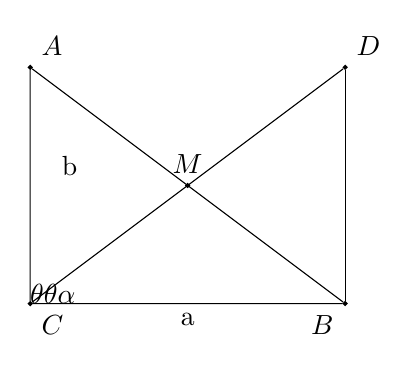
\begin{tikzpicture}
[scale=1,>=stealth,point/.style={draw,circle,fill = black,inner sep=0.5pt},]

%Triangle sides
\def\a{4}
\def\b{3}
\def\c{sqrt(\a^2+\c^2)}



%Labeling points
\node (A) at (0,\b)[point,label=above right:$A$] {};
\node (B) at (\a, 0)[point,label=below left:$B$] {};
\node (C) at (0, 0)[point,label=below right:$C$] {};
\node (M) at (\a*0.5,\b*0.5)[point,label=above:$M$] {};
\node (D) at (\a,\b)[point,label=above right:$D$] {};


%Drawing triangle ABC
\draw (A) -- node[left] {$\textrm{}$} (B) -- node[below] {$\textrm{a}$} (C) -- node[above,xshift=5mm] {$\textrm{b}$} (A);

%Joining CD
\draw (C)--(D);
%Joining BD
\draw (B)--(D);

%Drawing and marking angles
\tkzMarkAngle[fill=orange!40,size=0.5cm,mark=](A,M,C)
\tkzMarkAngle[fill=orange!40,size=0.5cm,mark=](B,M,D)
\tkzMarkAngle[fill=green!40,size=0.5cm,mark=](A,B,C)
\tkzMarkRightAngle[fill=blue!20,size=.2](A,C,B)
\tkzMarkRightAngle[fill=blue!20,size=.2](D,B,C)
\tkzLabelAngle[pos=0.65](A,M,C){$\theta$}
\tkzLabelAngle[pos=0.65](B,M,D){$\theta$}
\tkzLabelAngle[pos=0.65](A,B,C){$\alpha$}


\end{tikzpicture}
}
\caption{}
\label{fig:8.1.28}	
\end{figure}
%
%
%\renewcommand{\thefigure}{\theenumi}
%
%\item List the design parameters for construction
%\label{const:table1}
%\\
%\solution See Table. \ref{table:table1}. 
%%
%\begin{table}[ht!]
%\centering
%%\begin{tabular}{ |p{3cm}|p{3cm}|  }
%%\hline
%% \multicolumn{2}{|c|}{Initial Input Values.} \\
%%\hline
%%a & 4\\
%%\hline
%%b & 3\\
%%\hline
%%$\phase{(ACB)$ & $90^{\circ}$ \\
%%\hline
%%\end{tabular}
%%%%%%%%%%%%%%%%%%%%%%%%%%%%%%%%%%%%%%%%%%%%%%%%%%%%%%%%%%%%%%%%%%%%%%%
%%                                                                  %%
%%  This is the header of a LaTeX2e file exported from Gnumeric.    %%
%%                                                                  %%
%%  This file can be compiled as it stands or included in another   %%
%%  LaTeX document. The table is based on the longtable package so  %%
%%  the longtable options (headers, footers...) can be set in the   %%
%%  preamble section below (see PRAMBLE).                           %%
%%                                                                  %%
%%  To include the file in another, the following two lines must be %%
%%  in the including file:                                          %%
%%        \def\inputGnumericTable{}                                 %%
%%  at the beginning of the file and:                               %%
%%        \input{name-of-this-file.tex}                             %%
%%  where the table is to be placed. Note also that the including   %%
%%  file must use the following packages for the table to be        %%
%%  rendered correctly:                                             %%
%%    \usepackage[latin1]{inputenc}                                 %%
%%    \usepackage{color}                                            %%
%%    \usepackage{array}                                            %%
%%    \usepackage{longtable}                                        %%
%%    \usepackage{calc}                                             %%
%%    \usepackage{multirow}                                         %%
%%    \usepackage{hhline}                                           %%
%%    \usepackage{ifthen}                                           %%
%%  optionally (for landscape tables embedded in another document): %%
%%    \usepackage{lscape}                                           %%
%%                                                                  %%
%%%%%%%%%%%%%%%%%%%%%%%%%%%%%%%%%%%%%%%%%%%%%%%%%%%%%%%%%%%%%%%%%%%%%%



%%  This section checks if we are begin input into another file or  %%
%%  the file will be compiled alone. First use a macro taken from   %%
%%  the TeXbook ex 7.7 (suggestion of Han-Wen Nienhuys).            %%
\def\ifundefined#1{\expandafter\ifx\csname#1\endcsname\relax}


%%  Check for the \def token for inputed files. If it is not        %%
%%  defined, the file will be processed as a standalone and the     %%
%%  preamble will be used.                                          %%
\ifundefined{inputGnumericTable}

%%  We must be able to close or not the document at the end.        %%
	\def\gnumericTableEnd{\end{document}}


%%%%%%%%%%%%%%%%%%%%%%%%%%%%%%%%%%%%%%%%%%%%%%%%%%%%%%%%%%%%%%%%%%%%%%
%%                                                                  %%
%%  This is the PREAMBLE. Change these values to get the right      %%
%%  paper size and other niceties.                                  %%
%%                                                                  %%
%%%%%%%%%%%%%%%%%%%%%%%%%%%%%%%%%%%%%%%%%%%%%%%%%%%%%%%%%%%%%%%%%%%%%%

	\documentclass[12pt%
			  %,landscape%
                    ]{report}
       \usepackage[latin1]{inputenc}
       \usepackage{fullpage}
       \usepackage{color}
       \usepackage{array}
       \usepackage{longtable}
       \usepackage{calc}
       \usepackage{multirow}
       \usepackage{hhline}
       \usepackage{ifthen}

	\begin{document}


%%  End of the preamble for the standalone. The next section is for %%
%%  documents which are included into other LaTeX2e files.          %%
\else

%%  We are not a stand alone document. For a regular table, we will %%
%%  have no preamble and only define the closing to mean nothing.   %%
    \def\gnumericTableEnd{}

%%  If we want landscape mode in an embedded document, comment out  %%
%%  the line above and uncomment the two below. The table will      %%
%%  begin on a new page and run in landscape mode.                  %%
%       \def\gnumericTableEnd{\end{landscape}}
%       \begin{landscape}


%%  End of the else clause for this file being \input.              %%
\fi

%%%%%%%%%%%%%%%%%%%%%%%%%%%%%%%%%%%%%%%%%%%%%%%%%%%%%%%%%%%%%%%%%%%%%%
%%                                                                  %%
%%  The rest is the gnumeric table, except for the closing          %%
%%  statement. Changes below will alter the table's appearance.     %%
%%                                                                  %%
%%%%%%%%%%%%%%%%%%%%%%%%%%%%%%%%%%%%%%%%%%%%%%%%%%%%%%%%%%%%%%%%%%%%%%

\providecommand{\gnumericmathit}[1]{#1} 
%%  Uncomment the next line if you would like your numbers to be in %%
%%  italics if they are italizised in the gnumeric table.           %%
%\renewcommand{\gnumericmathit}[1]{\mathit{#1}}
\providecommand{\gnumericPB}[1]%
{\let\gnumericTemp=\\#1\let\\=\gnumericTemp\hspace{0pt}}
 \ifundefined{gnumericTableWidthDefined}
        \newlength{\gnumericTableWidth}
        \newlength{\gnumericTableWidthComplete}
        \newlength{\gnumericMultiRowLength}
        \global\def\gnumericTableWidthDefined{}
 \fi
%% The following setting protects this code from babel shorthands.  %%
 \ifthenelse{\isundefined{\languageshorthands}}{}{\languageshorthands{english}}
%%  The default table format retains the relative column widths of  %%
%%  gnumeric. They can easily be changed to c, r or l. In that case %%
%%  you may want to comment out the next line and uncomment the one %%
%%  thereafter                                                      %%
\providecommand\gnumbox{\makebox[0pt]}
%%\providecommand\gnumbox[1][]{\makebox}

%% to adjust positions in multirow situations                       %%
\setlength{\bigstrutjot}{\jot}
\setlength{\extrarowheight}{\doublerulesep}

%%  The \setlongtables command keeps column widths the same across  %%
%%  pages. Simply comment out next line for varying column widths.  %%
\setlongtables

\setlength\gnumericTableWidth{%
	53pt+%
	53pt+%
0pt}
\def\gumericNumCols{2}
\setlength\gnumericTableWidthComplete{\gnumericTableWidth+%
         \tabcolsep*\gumericNumCols*2+\arrayrulewidth*\gumericNumCols}
\ifthenelse{\lengthtest{\gnumericTableWidthComplete > \linewidth}}%
         {\def\gnumericScale{\ratio{\linewidth-%
                        \tabcolsep*\gumericNumCols*2-%
                        \arrayrulewidth*\gumericNumCols}%
{\gnumericTableWidth}}}%
{\def\gnumericScale{1}}

%%%%%%%%%%%%%%%%%%%%%%%%%%%%%%%%%%%%%%%%%%%%%%%%%%%%%%%%%%%%%%%%%%%%%%
%%                                                                  %%
%% The following are the widths of the various columns. We are      %%
%% defining them here because then they are easier to change.       %%
%% Depending on the cell formats we may use them more than once.    %%
%%                                                                  %%
%%%%%%%%%%%%%%%%%%%%%%%%%%%%%%%%%%%%%%%%%%%%%%%%%%%%%%%%%%%%%%%%%%%%%%

\ifthenelse{\isundefined{\gnumericColA}}{\newlength{\gnumericColA}}{}\settowidth{\gnumericColA}{\begin{tabular}{@{}p{53pt*\gnumericScale}@{}}x\end{tabular}}
\ifthenelse{\isundefined{\gnumericColB}}{\newlength{\gnumericColB}}{}\settowidth{\gnumericColB}{\begin{tabular}{@{}p{53pt*\gnumericScale}@{}}x\end{tabular}}

\begin{tabular}[c]{%
	b{\gnumericColA}%
	b{\gnumericColB}%
	}

%%%%%%%%%%%%%%%%%%%%%%%%%%%%%%%%%%%%%%%%%%%%%%%%%%%%%%%%%%%%%%%%%%%%%%
%%  The longtable options. (Caption, headers... see Goosens, p.124) %%
%	\caption{The Table Caption.}             \\	%
% \hline	% Across the top of the table.
%%  The rest of these options are table rows which are placed on    %%
%%  the first, last or every page. Use \multicolumn if you want.    %%

%%  Header for the first page.                                      %%
%	\multicolumn{2}{c}{The First Header} \\ \hline 
%	\multicolumn{1}{c}{colTag}	%Column 1
%	&\multicolumn{1}{c}{colTag}	\\ \hline %Last column
%	\endfirsthead

%%  The running header definition.                                  %%
%	\hline
%	\multicolumn{2}{l}{\ldots\small\slshape continued} \\ \hline
%	\multicolumn{1}{c}{colTag}	%Column 1
%	&\multicolumn{1}{c}{colTag}	\\ \hline %Last column
%	\endhead

%%  The running footer definition.                                  %%
%	\hline
%	\multicolumn{2}{r}{\small\slshape continued\ldots} \\
%	\endfoot

%%  The ending footer definition.                                   %%
%	\multicolumn{2}{c}{That's all folks} \\ \hline 
%	\endlastfoot
%%%%%%%%%%%%%%%%%%%%%%%%%%%%%%%%%%%%%%%%%%%%%%%%%%%%%%%%%%%%%%%%%%%%%%

\hhline{|-|-}
	 \multicolumn{1}{|p{\gnumericColA}|}%
	{\gnumericPB{\centering}\gnumbox{Parameter}}
	&\multicolumn{1}{p{\gnumericColB}|}%
	{\gnumericPB{\centering}\gnumbox{Value}}
\\
\hhline{|--|}
	 \multicolumn{1}{|p{\gnumericColA}|}%
	{\gnumericPB{\centering}\gnumbox{a}}
	&\multicolumn{1}{p{\gnumericColB}|}%
	{\gnumericPB{\centering}\gnumbox{5}}
\\
\hhline{|--|}
	 \multicolumn{1}{|p{\gnumericColA}|}%
	{\gnumericPB{\centering}\gnumbox{b}}
	&\multicolumn{1}{p{\gnumericColB}|}%
	{\gnumericPB{\centering}\gnumbox{6}}
\\
\hhline{|--|}
	 \multicolumn{1}{|p{\gnumericColA}|}%
	{\gnumericPB{\centering}\gnumbox{c}}
	&\multicolumn{1}{p{\gnumericColB}|}%
	{\gnumericPB{\centering}\gnumbox{4}}
\\
\hhline{|--|}
	 \multicolumn{1}{|p{\gnumericColA}|}%
	{\gnumericPB{\centering}\gnumbox{d}}
	&\multicolumn{1}{p{\gnumericColB}|}%
	{\gnumericPB{\centering}\gnumbox{4}}
\\
\hhline{|-|-|}
\end{tabular}

\ifthenelse{\isundefined{\languageshorthands}}{}{\languageshorthands{\languagename}}
\gnumericTableEnd

%\caption{To construct $\triangle ACB$}
%\label{table:table1}	
%\end{table}
%\item
%	For simplicity, let the greek letter $\alpha = \phase{ B$.  We have the following definitions.
%\begin{equation}
%\label{eq:8.1.28_tri_trig_defs}
%\begin{matrix}
	%\sin \theta = \frac{b}{c} & 	\cos \theta = \frac{a}{c} \\
	%\tan \theta = \frac{c}{a} & \cot \theta = \frac{1}{\tan \theta} \\
	%\csc \theta = \frac{1}{\sin \theta} & \sec \theta = \frac{1}{\cos \theta}
	%\end{equation}
%
%\item Find the coordinates of the various points in Fig. \ref{fig:tri_right_angle}
%\label{const:tri_right_angle}
%\\
%
%\solution 
%
%The values are listed in 
%%\item List the  derived values.
%%\label{const:table2}
%%\\
%%\solution See  
%Table. \ref{table:table2} 
%\begin{table}[ht!]
%%\centering
%%\begin{tabular}{ |p{3cm}|p{3cm}|  }
%%\hline
%% \multicolumn{2}{|c|}{Derived Values.} \\
%%\hline
%%$\vec{M}$ & $$\begin{pmatrix}2\\1.5\end{pmatrix}$$\\						
%%\hline
%%$\vec{D}$ & $$\begin{pmatrix}4\\3\end{pmatrix} $$\\
%%\hline
%\input{./tables/inp1.tex}
%\caption{To construct $\triangle DBC$}
%\label{table:table2}
%
%\end{table}
%
%\item Draw Fig. \ref{fig:tri_right_angle}.	
%\\
%\solution The  following Python code generates Fig. \ref{fig:tri_sss_py}
%%
%\begin{lstlisting}
%codes/triangle.py
%\end{lstlisting}
%\begin{figure}[!ht]
%\centering
%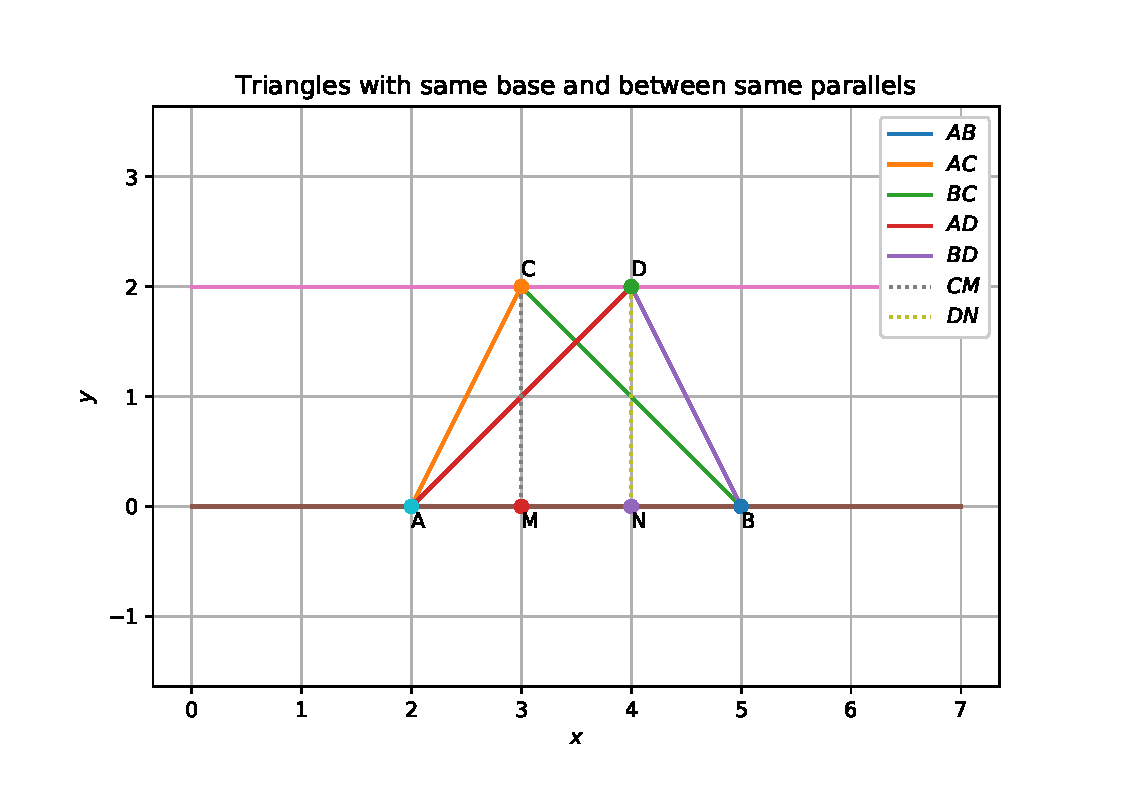
\includegraphics[width=\columnwidth]{./figs/triangle.eps}
%\caption{Triangle generated using python}
%\label{fig:tri_sss_py}
%\end{figure}
%
%%
%and the equivalent latex-tikz code generating Fig. \ref{fig:tri_right_angle} is 
%\begin{lstlisting}
%figs/triangle.tex
%\end{lstlisting}
%
%The above latex code can be compiled as a standalone document as
%\begin{lstlisting}
%figs/triangle_fig.tex
%\end{lstlisting}

%

%

%
%

%\end{enumerate}

%\renewcommand{\theequation}{\theenumi}
%\begin{enumerate}[label=\thesection.\arabic*.,ref=\thesection.\theenumi]
%\numberwithin{equation}{enumi}
	
\item {\em Proof: }
%\solution
From Fig. \ref{fig:8.1.28},	
%$\triangle AMC \cong \triangle DMB$  by SAS congruency $\because$
%\begin{enumerate}
%\item $AM = BM$
%\item $CM = DM$
%\item $\phase{AMC}$ = $\phase{DMB}$ ( Vertically Opposite Angles)
%\end{enumerate}
%
%\begin{figure}[!ht]
%\centering
%\resizebox{\columnwidth}{!}{

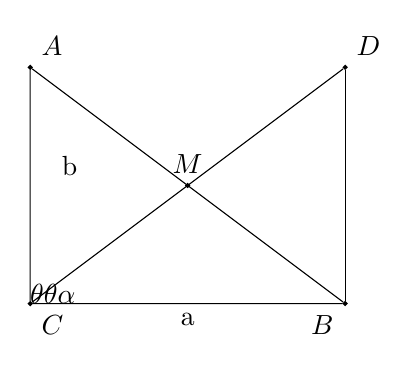
\begin{tikzpicture}
[scale=1,>=stealth,point/.style={draw,circle,fill = black,inner sep=0.5pt},]

%Triangle sides
\def\a{4}
\def\b{3}
\def\c{sqrt(\a^2+\c^2)}



%Labeling points
\node (A) at (0,\b)[point,label=above right:$A$] {};
\node (B) at (\a, 0)[point,label=below left:$B$] {};
\node (C) at (0, 0)[point,label=below right:$C$] {};
\node (M) at (\a*0.5,\b*0.5)[point,label=above:$M$] {};
\node (D) at (\a,\b)[point,label=above right:$D$] {};


%Drawing triangle ABC
\draw (A) -- node[left] {$\textrm{}$} (B) -- node[below] {$\textrm{a}$} (C) -- node[above,xshift=5mm] {$\textrm{b}$} (A);

%Joining CD
\draw (C)--(D);
%Joining BD
\draw (B)--(D);

%Drawing and marking angles
\tkzMarkAngle[fill=orange!40,size=0.5cm,mark=](A,M,C)
\tkzMarkAngle[fill=orange!40,size=0.5cm,mark=](B,M,D)
\tkzMarkAngle[fill=green!40,size=0.5cm,mark=](A,B,C)
\tkzMarkRightAngle[fill=blue!20,size=.2](A,C,B)
\tkzMarkRightAngle[fill=blue!20,size=.2](D,B,C)
\tkzLabelAngle[pos=0.65](A,M,C){$\theta$}
\tkzLabelAngle[pos=0.65](B,M,D){$\theta$}
\tkzLabelAngle[pos=0.65](A,B,C){$\alpha$}


\end{tikzpicture}
}
%\caption{}
%\label{fig:8.1.28}	
%\end{figure}
%\item From \eqref{eq:constr_b}, \eqref{eq:constr_c} and \eqref{eq:constr_d},
%%
%%
\begin{align}
\brak{\vec{D}-\vec{B}}^T
\brak{\vec{B}-\vec{C}} &= \myvec{0 & b}\myvec{a \\ 0} = 0
\\
\implies BD \perp BC
\end{align}
%%
%\item From \eqref{eq:constr_a}, \eqref{eq:constr_b}, \eqref{eq:constr_c} and \eqref{eq:constr_d},
\begin{align}
\norm{\vec{A}-\vec{B}} &= \norm{\myvec{-a \\ b}}
\\
\norm{\vec{C}-\vec{D}} &= \norm{\myvec{-a \\ -b}}
\\
\implies \norm{\vec{A}-\vec{B}} &= \norm{\vec{C}-\vec{D}}\\
\text{or, } AB &=CD
\label{eq:solution_abcd}
\end{align}
%%
Noting that BC is the common side, from RHS congruence,  $\triangle ACB \cong  \triangle DCB$.
\subitem  From \eqref{eq:solution_abcd}, noting that $\vec{M}$ is the mid point of both $AB$ and $CD$, 
\begin{align}
CM = \frac{1}{2}CD =\frac{1}{2} AB
\end{align}



%\end{enumerate}

\end{enumerate}
\fi

\item In an isosceles $\triangle ABC$, with $AB = AC$, the bisectors of $\angle B$ and $\angle C$ intersect each other at $O$. Join $A$ to $O$. Show that :
\begin{enumerate} 
\item $OB = OC$ 
\item $AO$ bisects $\angle A$
\end{enumerate}
\item In $\triangle ABC$, $AD$ is the perpendicular bisector of $BC$. Show that $\triangle ABC$ is an isosceles triangle in which $AB = AC$.
\item $ABC$ is an isosceles triangle in which altitudes $BE$ and $CF$ are drawn to equal sides $AC$ and $AB$ respectively . Show that these altitudes are equal.
%
\item $ABC$ is a triangle in which altitudes $BE$ and $CF$ to sides $AC$ and $AB$ are equal. Show that
%
\begin{enumerate} 
\item $\triangle  ABE \cong  \triangle  ACF $
\item  $AB = AC$, i.e., $ABC$ is an isosceles triangle.
\end{enumerate}
%
\item $ABC$ and $DBC$ are two isosceles triangles on the same base $BC$. Show that $\angle ABD = \angle ACD$.
%
\item  $\triangle  ABC$ and $\triangle  DBC$ are two isosceles triangles on the same base $BC$ and vertices $A$ and $D$ are on the same side of $BC$. If $AD$ is extended to intersect $BC$ at $P$, show that
\begin{enumerate}
\item $\triangle  ABD \cong  \triangle  ACD $
\item $\triangle  ABP \cong  \triangle  ACP $
\item $AP$ bisects $\angle  A$ as well as $\angle  D$. 
\item $AP$ is the perpendicular bisector of $BC$.
\end{enumerate}
\item $AD$ is an altitude of an isosceles $\triangle ABC$ in which $AB = AC$. Show that 
\begin{enumerate}
\item $AD$ bisects $BC$
\item $AD$ bisects $\angle  A$. 
\end{enumerate}

\item  Two sides $AB$ and $BC$ and median $AM$ of one triangle $ABC$ are respectively equal to sides $PQ$ and $QR$ and median $PN$ of $\triangle  PQR$. Show that: 
\begin{enumerate}
\item $\triangle  ABM \cong  \triangle  PQN $
\item $\triangle  ABC \cong  \triangle  PQR$
\end{enumerate}
\iffalse
\begin{enumerate}

%\renewcommand{\thefigure}{\theenumi.\arabic{figure}}
\begin{figure}[!ht]
\centering
\resizebox{\columnwidth}{!}{%\documentclass{article}
%\usepackage[utf8]{inputenc}
%\usepackage{tikz}
%\usepackage{tkz-euclide}
%\begin{document}

\begin{tikzpicture}
[scale=1,>=stealth,point/.style={draw,circle,fill = black,inner sep=0.5pt},]

%Triangle ABC
\def\a{6}
\def\b{4}
\def\c{5}
 
%Coordinates of A
%\def\p{(\a^2 + \c^2 - \b^2)/ (2*\a)}
\def\p{45/12}
\def\q{{sqrt(\c^2-\p^2)}}

%Labeling points
\node (A) at (\p,\q)[point,label=above right:$A$] {};
\node (B) at (0, 0)[point,label=below left:$B$] {};
\node (C) at (\a, 0)[point,label=below right:$C$] {};

%Foot median AM

\node (M) at (\a/2,0)[point,label=above right:$M$] {};

%Drawing triangle ABC
\draw (A) -- node[left] {$\textrm{c}$} (B) -- node[below] {$\textrm{a}$} (C) -- node[above,xshift=2mm] {$\textrm{b}$} (A);

%Drawing median AM
\draw (A) -- node[left] {$\textrm{}$}(M);

%Drawing and marking angles
\tkzMarkAngle[fill=orange!40,size=0.5cm,mark=](C,B,A)
\tkzLabelAngle[pos=-0.9](A,B,C){$\alpha$}

\end{tikzpicture}

\begin{tikzpicture}
[scale=1,>=stealth,point/.style={draw,circle,fill = black,inner sep=0.5pt},]

%Triangle PQR
\def\p{6}
\def\q{4}
\def\r{5}
 
%Coordinates of P
%\def\x{(\p^2 + \r^2 - \q^2)/ (2*\p)}
\def\x{45/12}
\def\z{{sqrt(\r^2-\x^2)}}

%Labeling points
\node (P) at (\x,\z)[point,label=above right:$P$] {};
\node (Q) at (0, 0)[point,label=below left:$Q$] {};
\node (R) at (\p, 0)[point,label=below right:$R$] {};

%Foot of median

\node (N) at (\p/2,0)[point,label=above right:$N$] {};

%Drawing triangle PQR
\draw (P) -- node[left] {$\textrm{r}$} (Q) -- node[below] {$\textrm{p}$} (R) -- node[above,xshift=2mm] {$\textrm{q}$} (P);

%Drawing median PN
\draw (P) -- node[left] {$\textrm{}$}(N);

%Drawing and marking angles
\tkzMarkAngle[fill=orange!40,size=0.5cm,mark=](R,Q,P)
\tkzLabelAngle[pos=-0.9](P,Q,R){$\theta$}

\end{tikzpicture}
%\end{document}
}
\caption{$\triangle ABC$ and $\triangle PQR$ by Latex-Tikz}
\label{fig:8.1.36_triangle_latex}	
\end{figure}
%
%
%\renewcommand{\thefigure}{\theenumi}
%

\item {\em Construction: }The coordinates of the various points of triangle ABC in Fig. \ref{fig:8.1.36_triangle_latex} are
%\label{}
%
\begin{align}
\vec{B} &= \myvec{0\\0} ,
\label{eq:8.1.36_constr_b}
\\
 \vec{C} &= \myvec{a\\0}, 
\label{eq:8.1.36_constr_c}
\end{align}

$\because \vec{M}$ is the midpoint of $BC$,
\begin{align}
\vec{M}= \frac{\vec{B}+\vec{C}}{2} =\myvec{a/2\\0},
\label{eq:8.1.36_constr_m}
\end{align}
%
$\triangle PQR$ is a horizontal translation of $\triangle ABC$.  Hence, if 
\begin{align}
\vec{Q}= \myvec{q\\0},
\label{eq:8.1.36_constr_q}
\end{align}
\begin{align}
\vec{P}= \vec{A} + \vec{Q}
\\
\vec{R}= \vec{C} + \vec{Q}
\end{align}

%




%\noindent a) \\
    In $\triangle ABM$  and  $\triangle PQN$ \newline 
    AB = PQ (Given)  \newline
    AM = PN (Given) \newline
    Since M and N are midpoints and BC = QR , \newline
    BM = QR  \newline
    :. By SSS congruence rule , $\triangle ABM \cong \triangle PQN$  \newline
    
        This implies that $\angle ABM = \angle PQN$ i.e $\alpha = \theta$
    \newline
    \\
    \\
b) \\   
Now in $\triangle ABC$  and  $\triangle PQR$ \newline 
AB = PQ (Given)  \newline
$\alpha = \theta$ \newline
BC = QR (Given)\newline
:. By SAS congruence rule , $\triangle ABC \cong \triangle PQR$ 
    



\end{enumerate}
\fi

\item  $BE$ and $CF$ are two equal altitudes of a triangle $ABC$. Using RHS congruence rule, prove that the triangle $ABC$ is isosceles.
\item  $ABC$ is an isosceles triangle with $AB = AC$. Draw $AP \perp BC$ to show that $\angle  B = \angle  C$.
%
\item $\triangle ABC$ is an isosceles triangle in which $AB = AC$. Side $BA$ is produced to $D$ such that $AD = AB$. Show that $\angle BCD$ is a right angle.
%
\item $ABC$ is a right angled triangle in which $\angle A$ = 90$\degree$ and $AB = AC$. Find $\angle B$ and $\angle C$.
%
\item Show that in a right angled triangle, the hypotenuse is the longest side.
\item Sides AB and AC of $\triangle  ABC$ are extended to points P and Q respectively. Also, $\angle  PBC < \angle  QCB$. Show that $AC > AB$.

\item Line segments $AD$ and $BC$ intersect at $O$ and form $\triangle OAB$ and $\triangle ODC$. $\angle  B < \angle  A$ and $\angle  C < \angle  D$. Show that $AD < BC$.

\item $AB$ and $CD$ are respectively the smallest and longest sides of a quadrilateral $ABCD$. Show that $\angle  A > \angle  C$ and $\angle  B > \angle  D$.
%
\item In $\triangle PQR,  PR > PQ$ and $PS$ bisects $\angle  QPR$. Prove that $\angle  PSR > \angle  PSQ$.
%
	\iffalse
\begin{enumerate}

\begin{figure}[!ht]
\centering
\resizebox{\columnwidth}{!}{\begin{tikzpicture}[scale = 1.5,>=stealth,point/.style={draw,circle,fill=black, inner sep=0.5pt},]

\node (Q) at (0, 0)[point,label=below left:$Q$] {};
\node (R) at (6, 0)[point,label=below right:$R$] {};
\node (P) at (2.25, 3.307189138830738)[point,label=above right:$P$] {};
\node (S) at (8/3, 0)[point,label=below:$S$] {};
\node (G) at (4/3, 0)[label=below:$y$] {};

\draw (P) -- node[below=5pt]{}(Q) -- (R) -- (P) -- (S);

\tkzMarkAngle[fill=green!20, mark=|](Q,P,S)
\tkzMarkAngle[fill=green!20, mark=|](S,P,R)

\end{tikzpicture}}
\caption{}
\label{fig:8.1.45_triangle1}	
\end{figure}

\item {\em Construction: } See Fig. \ref{fig:8.1.45_triangle1}.  The input parameters are
\begin{align}
\vec{P} &= \myvec{p\\q},
%\label{eq:constr_a} 
 \vec{Q} &= \myvec{0\\0}, 
\label{eq:constr_b}
\\
\vec{R} &= \myvec{a\\0},
%\label{eq:constr_c}
\label{eq:constr_d}
\end{align}
%
where $\vec{P}$  is obtained by choosing $PR > PQ$.
$\because PS$ is the angle bisector, its equation is given by (see Problem \ref{prob:8.1.23})
%
\begin{align}
PS: \vec{x} = \vec{P} + \lambda\brak{\frac{\vec{P}-\vec{Q}}{\norm{\vec{P}-\vec{Q}}}+\frac{\vec{P}-\vec{R}}{\norm{\vec{P}-\vec{R}}}}
\end{align}
%
$\vec{S}$ is obtained as the intersection of $PS$ and $QR$.



\item {\em Proof: } From the given information,
\begin{align}
\phase{Q} &> \phase{R}
\\
\implies \phase{Q} + \phase{SPQ}&> \phase{R}+  \phase{SPR} 
\\
\implies  \phase{PSQ}&>   \phase{PSR} 
\end{align}
$\because PS$ is the angle bisector.

\end{enumerate}
\fi

\item Show that of all line segments drawn from a given point not on it, the perpendicular line segment is the shortest.
%
\item $ABCD$ is a trapezium with $AB  \parallel  DC$. $E$ and $F$ are points on non-parallel sides $AD$ and $BC$ respectively such that $EF$ is parallel to $AB$
. Show that
$\frac{AE}{ED}=\frac{ BF}{  FC}$ .
\iffalse
\begin{enumerate}
\begin{figure}[!ht]
\centering
\resizebox{\columnwidth}{!}{%Exercise 8.1 prob 47
\begin{tikzpicture}
[scale=0.5,>=stealth,point/.style={draw,circle,fill = black,inner sep=0.5pt},]
%\tikzset{shift={(-3,0)}}
%Triangle sides
\def\a{4}
\def\c{9}
\def\xA{4}
\def\h{3}
\def\k{1}
%\def\c{7.5}
\def\yE{\h/2}
%Labeling points
\node (D) at (0,0)[point,label=below left:$D$] {};
\node (B) at ({\xA+\a}, \h )[point,label=above right:$B$] {};
\node (C) at (\c, 0)[point,label=below right:$C$] {};
%\node (E) at (2, \yE)
%\node (F) at (8.5, \yE)[point,label=below right:$F$] {};
%\node (M) at (\xA,\yE)[point,label=above right:$M$] {};
%\node (N) at ({\xA+\a}, \yE)[point,label=above left:$N$] {};
%\node (X) at (\xA , 0)[point,label=below left:$X$] {};
%\node (Y) at ({\xA+\a}, 0)[point,label=below right:$Y$] {};
\node (A) at (\xA , \h)[point,label=above left:$A$] {};
\node (E) at ($(D)!0.5!(A)$)[point,label=above left:$E$] {};
\node (F) at ($(B)!0.5!(C)$)[point,label=above right:$F$] {};



%A



%Drawing parallelogram ABCD
\draw (A) -- (B)--(C) --(D)--(A);
%\draw (A) --(X);
\draw (E) --(F);
\draw(A)--node[right]{$\textrm{k}$} (E)--node[right]{$\textrm{1}$} (D);
\draw(B)--node[left]{$\textrm{m}$} (F)--node[left]{$\textrm{1}$} (C);


%\draw (B) --(Y);
%marking right angles
%\tkzMarkRightAngle[fill=green!20,size=.2](D,X,A)
%\tkzMarkRightAngle[fill=green!20,size=.2](C,Y,B)


%
\end{tikzpicture}
}
\caption{}
\label{fig:8.1.47_trapezium_ABCD}	
\end{figure}

\item {\em Construction: }See Fig. \ref{fig:8.1.47_trapezium_ABCD}.
The input parameters are
\begin{align}
\label{eq:8.1.47_constr_d}
\vec{D} &= \myvec{0\\0} 
\\
\vec{C} &= \myvec{c\\0} 
\\
\vec{A} &= \myvec{p\\q} 
\\
\vec{B} &= \myvec{b\\q}, \quad b < c 
\label{eq:8.1.47_constr_c}
\end{align}
%
For $0 < k < 1$, 
\begin{align}
\label{eq:8.1.47_constr_e}
\vec{E} &= \frac{{k\vec{D} +\vec{A}}}{k+1}
\\
\vec{F} &= \frac{{k\vec{C} +\vec{B}}}{k+1}
\label{eq:8.1.47_constr_f}
\end{align}


\item {\em Proof: }Let 
\begin{align}
\vec{F} &= \frac{{{m\vec{C}} +\vec{B}}}{m+1}
\end{align}
%
From \eqref{eq:8.1.47_constr_e}
\begin{align}
\vec{E} &= \frac{{{k\vec{D}} +\vec{A}}}{k+1}
\\
\implies \vec{E} - \vec{F} &= \frac{{{k\vec{D}} +\vec{A}}}{k+1}-\frac{{{m\vec{C}} +\vec{B}}}{m+1}
\label{eq:8.1.47_sol_EF}
\\
& = \frac{\vec{A}}{k+1}-\frac{{{m\vec{C}} +\vec{B}}}{m+1}
\label{eq:8.1.47_sol_EF2}
\end{align}
$\because D = \vec{0}$.
\begin{align}
\because AB &\parallel BC, 
\\
\vec{C}-\vec{D} &= l\brak{\vec{B}-\vec{A}}
\\
\implies \vec{C} &= l\brak{\vec{B}-\vec{A}}
\label{eq:8.1.47_sol_C}
\end{align}
%
Substituting \eqref{eq:8.1.47_sol_C} in \eqref{eq:8.1.47_sol_EF2},
\begin{align}
 \vec{E} - \vec{F} &= \frac{\vec{A}}{k+1}-\frac{{{ml\brak{\vec{B}-\vec{A}}} +\vec{B}}}{m+1}
\\
 &= \vec{A}\brak{\frac{1}{k+1} + \frac{lm}{m+1}} - \vec{B}\brak{\frac{ml+1}{m+1}}
\label{eq:8.1.47_sol_EFinAB}
\end{align}
But $ EF \parallel AB$. So, for some w
\begin{align}
\implies \vec{E} - \vec{F} = w\brak{\vec{A}-\vec{B}}
\label{eq:8.1.47_sol_EFinAB2}
\end{align}
%
Comparing \eqref{eq:8.1.47_sol_EFinAB2} and \eqref{eq:8.1.47_sol_EFinAB}. We have
\begin{align}
\frac{1}{k+1} + \frac{lm}{m+1} &= \frac{ml+1}{m+1} = w
\\
\implies m+1+\brak{k+1}lm &= \brak{lm+1}\brak{k+1} 
\label{eq:8.1.47_sol_sol}
\\
\text{or, } m &=k
\end{align}

\end{enumerate}
\fi

\item $ST$ is a line joining two points on $PQ$ and $PR$ in $\triangle PQR$.  If $\frac{PS}{ SQ}=\frac{PT}{ TR}$ and $ \angle  PST = \angle  PRQ$, prove that $PQR$ is an isosceles triangle.
%
\item If $LM  \parallel  CB$ and $LN  \parallel  CD$, prove that $\frac{AM}{AB} = \frac{ AN}{AD}$.
%
\item $D$ is a point on $AB$ and $E, F$ are points on $BC$ such that $DE  \parallel  AC$ and $DF  \parallel  AE$. Prove that $\frac{BF} {FE} =\frac{BE}  {EC}$.
%
\item $O$ is a point in the interior of $\triangle ABC$. $D$ is a point on $OA$.  If $DE  \parallel  OB$ and $DF  \parallel  OC$. Show that $EF  \parallel  BC$.
	\iffalse
\begin{enumerate}
\begin{figure}[!ht]
\centering
\resizebox{\columnwidth}{!}{\begin{tikzpicture}
[scale=2,>=stealth,point/.style={draw,circle,fill = black,inner sep=0.5pt},]

%Triangle sides
\def\a{5}
\def\b{6}
\def\c{4}
 
%Coordinates of A
\def\p{0.5}
\def\q{{sqrt(\c^2-\p^2)}}

%Labeling points
\node (A) at (\p,\q)[point,label=above right:$A$] {};
\node (B) at (0, 0)[point,label=below left:$B$] {};
\node (C) at (\a, 0)[point,label=below right:$C$] {};
\node (O) at (2,1.5)[point,label=below:$O$]{};
%Foot of median

\node (D) at ($(A)!0.5!(O)$)[point,label=below:$D$] {};
\node (E) at ($(A)!0.5!(B)$)[point,label=left:$E$] {};
\node (F) at ($(C)!0.5!(A)$)[point,label=right:$F$] {};

%Drawing triangle ABC
\draw (A) -- node[left, xshift=-5mm,yshift=5mm] {$\textrm{c}$} (B) -- node[below, yshift=-5mm] {$\textrm{a}$} (C) -- node[above right,xshift=2mm,yshift=5mm] {$\textrm{b}$} (A);
\draw (A) -- (D) -- (O);
%Drawing medians BE and CF
\draw (D) -- (E);
\draw (D) -- (F);
\draw (O) -- (B);
\draw (O) -- (C);
%Drawing EF
\draw (E) -- (F);

%Labeling sides
%\node [right] at ($(A)!0.5!(E)$) {$\frac{b}{2}$};
%\node [right] at ($(C)!0.5!(E)$) {$\frac{b}{2}$};
%\node [left] at ($(B)!0.5!(F)$) {$\frac{c}{2}$};
%\node [left] at ($(A)!0.5!(F)$) {$\frac{c}{2}$};




%Angles
\tkzMarkAngle[size=.3](D,E,A)
\tkzMarkAngle[size=.3](O,B,A)
%
\tkzMarkAngle[size=.7](A,F,D)
\tkzMarkAngle[size=.7](A,C,O)
%%
\tkzMarkAngle[size=.2](A,D,E)
\tkzMarkAngle[size=.2](A,O,B)
%%
\tkzMarkAngle[size=.2](F,D,A)
\tkzMarkAngle[size=.2](C,O,A)
%
%\tkzMarkAngle[size=.3](E,A,D)
%\tkzMarkAngle[size=.3](D,A,F)

\begin{comment}
%Angles
\tkzMarkAngle[fill=green!60,size=.3](D,E,A)
\tkzMarkAngle[fill=green!60,size=.3](O,B,A)
%
\tkzMarkAngle[fill=red!60,size=.5](A,F,D)
\tkzMarkAngle[fill=red!60,size=.5](A,C,O)
%%
\tkzMarkAngle[fill=yellow!60,size=.2](A,D,E)
\tkzMarkAngle[fill=yellow!60,size=.2](A,O,B)
%%
\tkzMarkAngle[fill=orange!60,size=.2](F,D,A)
\tkzMarkAngle[fill=orange!60,size=.2](C,O,A)
%
\tkzMarkAngle[fill=blue!60,size=.3](E,A,D)
\tkzMarkAngle[fill=blue!60,size=.3](D,A,F)
\end{comment}
\end{tikzpicture}
}
\caption{}
\label{fig:8.1.51_similar}	
\end{figure}
\item {\em Construction: }
See Fig. \ref{fig:8.1.51_similar}. The input values are
\begin{align}
     \vec{B}= \myvec{0\\0}
    \vec{C}=\myvec{a\\0}
    \vec{A}=\myvec{p\\q}
\end{align}

\subitem The point inside $\triangle ABC$ is generated as
\begin{align}
\vec{O} &= \lambda_1 \brak{\vec{B}-\vec{A}} +  \lambda_2 \brak{\vec{B}-\vec{C}}
\\
0 &< \lambda_1  < 1,
\\
0 &< \lambda_2  < 1,
\\
0 &< \lambda_1+\lambda_2  < 1,
\end{align}
%
by choosing appropriate values of $\lambda_1, \lambda_2$.
\subitem Determination of points D,E and F.
\begin{align}
\vec{D} = \frac{k\vec{A} + \vec{O}}{k+1}, \quad 0 < k < 1
\end{align}
%
where $k$ is an input parameter.
\begin{align}
\because DE &\parallel OB, DF \parallel OC,
\\
\begin{split}
\vec{E} &= \frac{k\vec{A} + \vec{B}}{k+1}, 
\\
\vec{F} &= \frac{k\vec{A} + \vec{C}}{k+1}, 
\end{split}
\label{eq:8.1.51_ef}
\end{align}

\item {\em Proof: }
From \eqref{eq:8.1.51_ef}
\begin{align}
\vec{E} - \vec{F} &= \frac{\vec{B}-\vec{C}}{k+1}, 
\\
\implies EF &\parallel BC
\end{align}


\end{enumerate}
\fi

\item $O$ is a point in the interior of $\triangle PQR$.  $A, B and C$ are points on $OP, OQ$ and $OR$ respectively such that $AB  \parallel  PQ$ and $AC  \parallel  PR$. Show that $BC  \parallel  QR$.
%
\item $ABCD$ is a trapezium in which $AB  \parallel  DC$ and its diagonals intersect each other at the point $O$. Show
that
$\frac{AO}{ BO}=\frac{CO}{  DO}$
%
\item The diagonals of a quadrilateral $ABCD$ intersect each other at the point $O$ such that $\frac{AO}{ BO}=\frac{CO}{  DO}$.   Show that $ABCD$ is a trapezium.
%
\item $PQ \parallel RS$ and $PS$ intersects $QR$ at $O$.  Show that $\triangle OPQ \sim \triangle ORS$.
 \item $CM$ and $RN$ are respectively the medians of $ \triangle  ABC$ and $ \triangle  PQR$. If $ \triangle  ABC  \sim   \triangle  PQR$, prove that 
\begin{enumerate}
\item  $ \triangle  AMC  \sim   \triangle  PNR$ 
\item  $\frac{CM}{RN}=\frac{ AB}{  PQ}$
\item $ \triangle  CMB  \sim   \triangle  RNQ$
%
\end{enumerate}
\item Diagonals $AC$ and $BD$ of a trapezium $ABCD$ with $AB  \parallel  DC$ intersect each other at the point $O$. Using a similarity criterion for two triangles, show that
$\frac{OA}{OC} =  \frac{OB}  {OD}$
%
\item In $\triangle PQR$, $QP$ is extended to $T$ and $S$ is a point on $QR$ such that $ \frac{QR}{QS}=\frac{ QT}{  PR}$. If $\angle PRQ = \angle PQS$, show that 
 that  $\triangle  PQS  \sim   \triangle  TQR$.
\item $S$ and $T$ are points on sides $PR$ and $QR$ of $\triangle PQR$ such that $\angle P = \angle 
 RTS$. Show that $\triangle RPQ \sim \triangle RTS$.
\item  In $\triangle ABC$, $D$ and $E$ are points on the sides $AB$ and $AC$ respectively.  If  $\triangle  ABE \cong   \triangle  ACD$, show that  $\triangle  ADE  \sim   \triangle  ABC$.
\item   Altitudes $AD$ and CE of  $\triangle  ABC$ intersect each other at the point $P$. Show that:
%
\begin{enumerate}
\item   $\triangle  AEP  \sim   \triangle  CDP $
\item   $\triangle  ABD  \sim   \triangle  CBE $
\item   $\triangle  AEP  \sim   \triangle  ADB$
 \item  $\triangle  PDC  \sim   \triangle  BEC$
\end{enumerate}
%
\item  $E$ is a point on the side $AD$ produced of a parallelogram $ABCD$ and $BE$ intersects $CD$ at $F$. Show that  $\triangle  ABE  \sim   \triangle  CFB$.
\item  $ABC$ and $AMP$ are two right triangles, right angled at $B$ and $M$ respectively. $M$ lies on $AC$ and $AB$ is extended to meet $P$. Prove that: 
\begin{enumerate}
\item   $\triangle  ABC  \sim   \triangle  AMP$
\item  $\frac{CA}{PA} = \frac{BC}{  MP}$
\end{enumerate}
%
\item  $CD$ and $GH$ are respectively the bisectors of  $\angle  ACB$ and  $\angle  EGF$ such that $D$ and $H$ lie on sides $AB$ and $FE$ of  $\triangle  ABC$ and  $\triangle  EFG$ respectively. If  $\triangle  ABC  \sim   \triangle  FEG$, show that:
\item  $\frac{CD}{GH} = \frac{ AC}{  FG}$
\item  $ \triangle  DCB  \sim   \triangle  HGE$
 \item  $ \triangle  DCA  \sim   \triangle  HGF$
\item  $E$ is a point on side $CB$ produced of an isosceles $\triangle ABC$ with $AB = AC$. If $AD  \perp  BC$ and $EF  \perp  AC$, prove that  $\triangle  ABD  \sim   \triangle  ECF$.
\item  Sides $AB$ and $BC$ and median $AD$ of a $\triangle ABC$ are respectively proportional to sides  $PQ$  and $QR$ and median $PM$ of  $\triangle PQR$. Show that  $\triangle  ABC  \sim  \triangle PQR$ .
\item  $D$ is a point on the side $BC$ of a $\triangle ABC$ such that  $\angle  ADC =  \angle  BAC$. Show that $CA^2 = CB.CD$.
\item  Sides $AB$ and $AC$ and median $AD$ of a $\triangle ABC$ are respectively proportional to sides $PQ$ and $PR$ and median $PM$ of another $\triangle PQR$. Show that  $\triangle  ABC  \sim   \triangle PQR$ .%
\item  If $AD$ and $PM$ are medians of $\triangle s ABC$ and $PQR$, respectively where  $\triangle  ABC  \sim   \triangle PQR$ , prove that
$\frac{AB}{ PQ} = \frac{AD}{  PM}$
\item The line segment $XY$ is parallel to side $AC$ of  $\triangle  ABC$ and it divides the triangle into two parts of equal areas. Find the ratio
$\frac{AX}{ AB}$
% 
\item  Diagonals of a trapezium $ABCD$ with $AB  \parallel  DC$ intersect each other at the point $O$. If $AB = 2 CD$, find the ratio of the areas of $\triangle s AOB$ and $COD$.
\item  $ABC$ and $DBC$ are two triangles on the same base $BC$. If $AD$ intersects $BC$ at $O$, show that
$\frac{ar (ABC)}{ ar (DBC)}=\frac{AO}{  DO}$.
\item  If the areas of two similar triangles are equal, prove that they are congruent.
\item  $D, E$ and $F$ are respectively the mid-points of sides $AB$, $BC$ and $CA$ of  $\triangle  ABC$. Find the ratio of the areas of  $\triangle  DEF$ and  $\triangle  ABC$.
\item  Prove that the ratio of the areas of two similar triangles is equal to the square of the ratio of their corresponding medians.
\item  Prove that the area of an equilateral triangle described on one side of a square is equal to half the area of the equilateral triangle described on one of its diagonals.
\item $ABC$ and $BDE$ are two equilateral triangles such that $D$ is the mid-point of $BC$. Find the ratio of the areas of triangles $ABC$ and $BDE$.
\item The sides of two similar triangles are in the ratio 4 : 9. Find the ratio the area of  these triangles are in the ratio
\item In $\triangle ABC, \angle  ACB = 90\degree$ and $CD  \perp  AB$. Prove that 
$\frac{BC^2}{AC^2} = \frac{BD}{ AD}$.
\item In $\triangle ABC$,  if $AD  \perp  BC$, prove that $AB^2+ CD^2 = BD^2 + AC^2$.
\item $BL$ and $CM$ are medians of a $\triangle ABC$ right angled at $A$. Prove that $4 (BL^2 + CM^2
) = 5 BC^2$ .
\item $O$ is any point inside a rectangle $ABCD$. Prove that $OB^2+OD^2 = OA^2+OC^2$.
\item  $PQR$ is a triangle right angled at $P$ and $M$ is a point on $QR$ such that $PM  \perp  QR$. Show that $PM^2= QM . MR$.
\item  $ABD$ is a triangle right angled at $A$ and $AC \perp  BD$. Show that
\begin{enumerate}
\item  $AB^2 = BC . BD$
\item  $AC^2 = BC . DC$
\item  $AD^2  = BD . CD$
\end{enumerate}
\item  $ABC$ is an isosceles triangle right angled at $C$. Prove that $AB^2= 2 AC^2$.
 \item  $ABC$ is an isosceles triangle with $AC = BC$. If $AB^2=2 AC^2$, prove that $ABC$ is a right triangle.
\item  $ABC$ is an equilateral triangle of side $2a$. Find each of its altitudes. 
\item  Prove that the sum of the squares of the sides of a rhombus is equal to the sum of the squares of its diagonals.
\item  $O$ is a point in the interior of a $\triangle ABC, OD  \perp  BC, OE  \perp  AC and OF  \perp  AB$. Show that
%
\begin{enumerate}
\item  $OA^2 + OB^2 + BD^2 – OD2 – OE2– OF2 = AF^2 + BD^2 + CE^2$.
\item  $AF^2 + BD^2 +CE^2 = AE^2 + CD^2 + BF^2$.
\end{enumerate}
\item  $D$ and $E$ are points on the sides $CA$ and $CB$ respectively of a $\triangle ABC$ right angled at $C$. Prove that $AE^2+ BD^2 = AB^2 + DE^2$.
\item  The perpendicular from $A$ on side $BC$ of a  $\triangle  ABC$ intersects $BC$ at $D$ such that $DB = 3 CD$. Prove that $2 AB^2= 2 AC^2 + BC^2$ .
\item  In an equilateral $\triangle ABC$, $D$ is a point on side $BC$ such that $BD = \frac{1}{3} BC$.  Prove that $9 AD^2= 7 AB^2$.
\item  In an equilateral triangle, prove that three times the square of one side is equal to four times the square of one of its altitudes.
\item  $PS$ is the bisector of  $\angle  QPR$ of  $\triangle PQR$ . Prove that
$\frac{QS}{SR} = \frac{PQ}{PR}$
\item $D$ is a point on hypotenuse $AC$ of  $\triangle  ABC$, such that $BD  \perp  AC, DM  \perp  BC$ and $DN  \perp  AB$. Prove that :
\begin{enumerate}
\item  DM2 = DN . MC  
 \item  DN2 = DM . AN
\end{enumerate}

\item  $ABC$ is a triangle in which  $\angle  ABC > 90\degree$ and $AD  \perp  CB$ produced. Prove that
$ AC^2= AB^2 + BC^2 + 2 BC . BD$.
\item $ABC$ is a triangle in which  $\angle  ABC < 90\degree$ and $AD  \perp  BC$. Prove that $AC^2= AB^2 + BC^2 – 2 BC . BD$.
\item $AD$ is a median of a $\triangle ABC$ and $AM  \perp  BC$. Prove that :
\begin{enumerate}
\item  $AC^2 = AD^2 + BC . DM +
\brak{\frac{BC}{ 2}}^2$
\item  $AB^2 = AD^2 – BC . DM + \brak{\frac{BC}{ 2}}^
2 $
\item  $AC^2 + AB^2 = 2 AD^2 + \frac{1}{ 2} BC^2$
\end{enumerate}
\item Prove that the sum of the squares of the diagonals of parallelogram is equal to the sum of the squares of its sides.
\item   $D$ is a point on side $BC$ of  $\triangle  ABC$ such that
$\frac{BD}{CD} \frac{AB}{AC}  $.  Prove that $AD$ is the bisector of  $\angle  BAC$.
\end{enumerate}


